\chapter{真空のエネルギーとド・ジッター地平線}

\lectureoverview{真空のエネルギーは通常の物質とは異なる。それは特別な慣性系を選び出すこともなく、宇宙の膨張に伴って薄まることもない。重力を含めると、一見無害に見えるこのエネルギーの零点が時空の幾何学を変える。物質優勢の法則 \(a(t)\propto t^{2/3}\) を導出し、それを真空優勢の法則 \(a(t)\propto e^{Ht}\) と対比し、次にド・ジッター時空を共形座標で書き直す。得られる因果図は、固有距離が固定された観測者依存の事象の地平線を明らかにする。}

\section{真空における量子揺らぎ}

本講義全体の動機となる問いから始めよう。量子場の理論は空っぽの空間にエネルギーを割り当てる。これは、実在の電子--陽電子対が絶えず無から現れているということを意味するのだろうか。

\begin{classroomqa}
\audiencequestion{電子--陽電子の生成と消滅は実際に真空で起こっているのか、それとも単なる帳簿上の操作にすぎないのか。\lecturetimestamp{00:00:06}}
\lecturerresponse{仮想対は真空のエネルギーに寄与するが、それらは空っぽの空間から現れるのを観察できる通常の粒子ではない。それらは量子基底状態の揺らぎであり、仮想過程にふさわしい制限の範囲内でのみ持続する。}
\end{classroomqa}

調和振動子が最も明快な模型を与える。古典的には、それはポテンシャルの最小点で静止したままでいられる。量子力学的には、最小点における正確な位置と正確にゼロの運動量は両立しない。基底状態は両者の間で妥協し、零点エネルギー
\begin{equation}
E_0=\frac{1}{2}\hbar\omega.
\label{eq:l08-zero-point}
\end{equation}
を保つ。これが振動子の持ちうる最小のエネルギーである。これは励起状態ではなく、観測可能な粒子の流れを表すものでもない。

自由場は規準モードに分解され、各モードは振動子のように振る舞う。空洞内の電磁場はよく知られた例である。すべてのモードが式~\eqref{eq:l08-zero-point}の形の項に寄与し、電子、クォーク、その他の量子場もそれぞれ独自の基底状態の揺らぎに寄与する。これらの寄与を足し合わせたものが、我々が真空のエネルギーと呼ぶものである。素朴な微視的見積もりと観測された宇宙論的スケールとの間の悪名高い不一致は実在するが、それは本講義の主題ではない。

\begin{classroomqa}
\audiencequestion{およそ \(120\) 桁の不一致について再び議論されるのだろうか。\lecturetimestamp{00:02:59}}
\lecturerresponse{ここでは扱わない。当面の目標は宇宙論的地平線を理解することである。すなわち、宇宙論の方程式がどのように加速膨張を生み出すのか、そしてなぜ加速膨張が事象の地平線を生み出すのかである。}
\end{classroomqa}

\begin{classroomqa}
\audiencequestion{前回の講義の紫外--赤外の関係は今夜の議論の一部なのだろうか。\lecturetimestamp{00:03:59}}
\lecturerresponse{後で再び取り上げるかもしれないが、予定された論証の一部ではない。当面の道筋は真空のエネルギーから宇宙論へ、そして地平線へと進む。}
\end{classroomqa}

\section{なぜ真空のエネルギーはローレンツ不変なのか}

次の問いは初歩的に見えるが、真空のエネルギーの定義的な性質を露わにする。もし空っぽの空間が正のエネルギー密度を持つなら、なぜそれは光学媒質のように振る舞い、光の速さを変えないのか。

\begin{classroomqa}
\audiencequestion{正の真空のエネルギー密度は屈折効果を持ち、光をわずかに遅く進ませるべきではないのか。\lecturetimestamp{00:04:35}}
\lecturerresponse{通常の物質はそれが可能である。なぜならそれは特別な静止系を定義するからである。真空のエネルギーは異なる。それはそのような系を選び出さず、すべての慣性観測者が同じ真空のエネルギー密度を得る。したがって光の局所的な測定は不変の速さ \(c\) を保つ。}
\end{classroomqa}

法則の対称性と特定の状態の対称性を区別しなければならない。物理学の方程式は並進不変でありえても、スタンフォードはバークリーではなく、地球は星間空間ではない。\emph{物理的配置全体}を並進させても法則は変わらない。物質の実際の配置は、あらゆる場所で同じに見える必要はない。同様に、回転不変な方程式はこの教室を回転対称にするものではない。

同じ区別がローレンツ変換にも当てはまる。気体には静止系がある。それを通り抜けて運動する観測者は運動する分子と異なるエネルギー密度を見るので、気体の状態は、それを支配する方程式がローレンツ不変であっても、ローレンツ不変ではない。通常の物質、放射浴、実験装置はすべて、特別な運動や方向を選び出すことによって対称性を破る。

真空のエネルギーは、そうしない例外的な形態の物質である。真空エネルギーの密度を報告する検出器を想像しよう。静止しているとき、それはある値\(\rho_{\rm vac}\)を与える。検出器を加速して測定を繰り返す。結果は変わらない。相対論的表記では、この性質は計量に比例する応力テンソルによって表される。
\begin{equation}
T_{\mu\nu}^{\rm vac}=-\rho_{\rm vac}g_{\mu\nu},
\qquad
p_{\rm vac}=-\rho_{\rm vac}.
\label{eq:l08-vacuum-stress}
\end{equation}
\editorialnote{圧力の関係は板書では導出されない。それは講義の二つの定義的性質、すなわちローレンツ不変性と膨張中の一定密度の背後にある共変的な言明である。}

局所的な但し書きが重要である。観測者のそばを通過する光線は、近くの時計と物差しで測ると\(c\)で進む。膨張する幾何学において、遠方の光線の私たちに対する速さを問うには、座標の選択と、遠く離れた事象を比較するための規定が必要である。その座標速度は\(c\)に等しい必要はない。すべての局所的な観測者が\(c\)を測定するとしても、である。

\begin{classroomqa}
\audiencequestion{この議論において、真空エネルギーと宇宙定数は同義ですか。\lecturetimestamp{00:11:57}}
\lecturerresponse{はい。それらはアインシュタイン方程式における同じ項の二つの配置である。幾何学の側では宇宙定数として記述され、源の側ではローレンツ不変な真空の応力エネルギーとして記述されうる。}
\end{classroomqa}

\section{何が薄まり、何が薄まらないか}

質量\(m\)の非相対論的粒子で大きな領域を満たす。銀河や銀河団を平均するのに十分大きなスケールでは、分布は一様であると仮定する。共動体積が\(N\)個の粒子を含むなら、その物質密度は
\begin{equation}
\rho_m=\frac{Nm}{V}.
\end{equation}
である。すべての線形の長さが二倍になると、体積は\(2^3=8\)倍に増えるが、\(N\)と\(m\)は変わらない。したがって密度は以前の値の八分の一に下がる。通常の物質が薄まるのは、同じ粒子がより大きな物理的体積を占めるからである。

輻射も薄まり、しかもより速く薄まる。その数密度は体積とともに下がり、一方で各光子の波長は引き伸ばされ、そのエネルギーは赤方偏移する。後に結果\(\rho_r\propto a^{-4}\)を記録するが、今夜は輻射優勢の宇宙論を解かない。

真空エネルギーは例外である。
\begin{equation}
\rho_{\rm vac}(t)=\text{constant}.
\label{eq:l08-rho-vac-constant}
\end{equation}
それは集団化せず、方向を選ばず、慣性系を選ばず、空間が膨張しても密度が小さくならない。共動する箱が大きくなれば、その中に含まれる真空エネルギーはその体積に比例して増える。

\editorialnote{一定密度とは、膨張する共動する箱の内部の全真空エネルギーが一定であることを意味しない。共変的な応力エネルギーの保存
\(\dot\rho+3H(\rho+p)=0\)は、真空エネルギーが負の圧力\(p_{\rm vac}=-\rho_{\rm vac}\)をもつために満たされる。仕事の項が、箱の全真空エネルギーの変化をちょうど供給する。}

\section{重力はエネルギーの零点を見る}

非重力の実験室物理学では、すべてのエネルギーを同じ定数だけずらしても通常は何も変わらない。スペクトルは差に依存する。励起した原子と励起していない原子の間のエネルギー、あるいは粒子がある状態とない状態の間のエネルギーである。空の空間は、その絶対エネルギーを測る基準を何も提供しないように見える。

重力は問いを変える。質量はエネルギーであり、エネルギーは重力の源であり、したがって真空エネルギーは重力を及ぼす。原子遷移では見えなかった定数が時空を曲げうる。

アインシュタイン方程式は幾何学と源を分ける。
\begin{equation}
G_{\mu\nu}=8\pi G_N T_{\mu\nu},
\label{eq:l08-einstein}
\end{equation}
ここで単位は\(c=1\)である。アインシュタインテンソル\(G_{\mu\nu}\)は計量\(g_{\mu\nu}(x)\)とその導関数から作られる。応力テンソル\(T_{\mu\nu}\)は、物質および非重力場からのエネルギー密度、運動量密度、圧力、応力を含む。真空エネルギーは通常の物質とまったく同様にこの源の側に属する。\editorialnote{口頭の導入は\(8\pi/3\)をテンソル方程式と簡単に結びつける。因子\(1/3\)は以下の空間的に平坦なフリードマン方程式に属し、式~\eqref{eq:l08-einstein}には属さない。}

\begin{figure}[htbp]
\centering
\includegraphics[width=0.62\textwidth]{lecture_08_figure_02.png}
\caption{時空計量\(g_{\mu\nu}(x)\)から作られるアインシュタイン方程式の幾何学の側。}
\lectureframe{00:21:58.820}
\end{figure}

\section{幾何学はスケール因子に還元される}

ここで、平坦な空間的断面をもつ最も単純な一様膨張幾何学を選ぶ。
\begin{equation}
ds^2=-dt^2+a(t)^2\,d\mathbf{x}^2,
\qquad
d\mathbf{x}^2=dx^2+dy^2+dz^2.
\label{eq:l08-frw-metric}
\end{equation}
座標の印\(\mathbf{x}\)は無限のゴムシートに描かれている。それらは動く必要はないが、それらの物理的間隔は動く。\(\Delta\mathbf{x}\)だけ離れた二つの共動点は、\(t\)を固定したとき固有距離
\begin{equation}
D(t)=a(t)\lvert\Delta\mathbf{x}\rvert.
\label{eq:l08-proper-distance}
\end{equation}
をもつ。したがって、この高度に対称な幾何学の時間依存性はすべて一つの関数、スケール因子\(a(t)\)に蓄えられる。\(a\)が一定なら、空間的再スケーリングの後で平坦なミンコフスキー時空を与える。\(a\)が時間に依存すれば、各空間的断面を平坦に保ちながら、時空全体を曲がったものにしうる。

\begin{classroomqa}
\audiencequestion{座標マーク\(x=7\)と\(x=13\)について、それらの座標間隔は\(4\)か。\lecturetimestamp{00:27:40}}
\lecturerresponse{いいえ。それは\(13-7=6\)であり、したがってそれらの物理的間隔は\(6a(t)\)である。この補正は有用である。\(x\)は共動位置を表し、一方\(a(t)\)を掛けると物理的距離が得られる。}
\end{classroomqa}

この計量と空間的に一様なエネルギー密度に対して、アインシュタイン方程式の一つの成分が空間的に平坦なフリードマン方程式となる。
\begin{equation}
\left(\frac{\dot a}{a}\right)^2
=\frac{8\pi G_N}{3}\rho(t).
\label{eq:l08-friedmann}
\end{equation}
比
\begin{equation}
H(t)\equiv\frac{\dot a(t)}{a(t)}
\label{eq:l08-hubble-definition}
\end{equation}
はハッブルパラメータである。これはこの段階では定義であり、時間とともに変化しうる。

\begin{figure}[htbp]
\centering
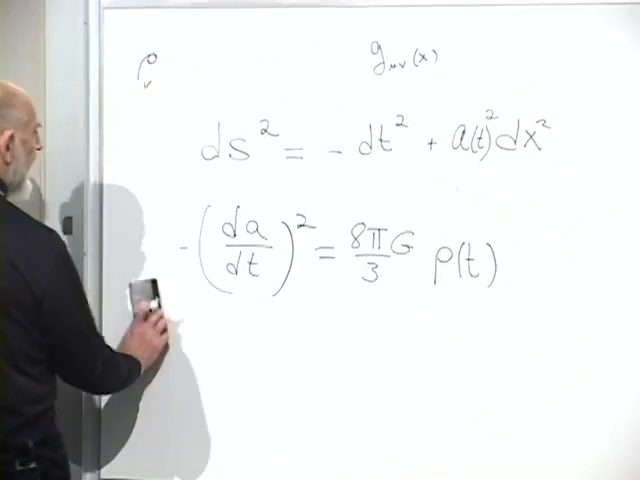
\includegraphics[width=0.90\textwidth]{lecture_08_figure_03.png}
\caption{黒板で欠けていた因子\(1/a^2\)が復元された後の、平坦膨張計量とフリードマン方程式。}
\lectureframe{00:30:30.000}
\end{figure}

\paragraph{エネルギー収支の描像。}
このエネルギー収支の描像に対して、式~\eqref{eq:l08-friedmann}は模式的に
\begin{equation}
-\frac{3}{8\pi G_N}H^2+\rho=0.
\label{eq:l08-energy-heuristic}
\end{equation}
と書ける。物質エネルギーは正であり、一方、膨張するスケール因子によって表される重力自由度は負の運動項を持つ。この縮約された問題では、負の重力エネルギーと正の物質エネルギーの和がゼロに等しいことが有用な記憶法である。

\editorialnote{式~\eqref{eq:l08-energy-heuristic}は高度に対称なミニスーパースペース模型におけるハミルトニアン拘束条件であり、任意の宇宙がゼロに等しい大域的に保存された全エネルギーを持つという座標に依存しない定理ではない。講義ではこれをフリードマン拘束条件のヒューリスティックな解釈として用いている。}

\section{物質優勢膨張}

座標の辺の長さが\(\Delta x=1\)である共動的な数学的箱に戻る。その物理的な辺の長さは\(a(t)\)であり、したがってその物理的体積は\(a(t)^3\)である。もし質量\(m\)の非相対論的粒子を\(N\)個含むならば、
\begin{equation}
\rho_m(t)=\frac{Nm}{a(t)^3}
=\frac{\rho_0}{a(t)^3}.
\label{eq:l08-matter-density}
\end{equation}
粒子自体は膨張しない。それらの平均間隔が膨張するのである。

\begin{figure}[htbp]
\centering
\includegraphics[width=0.84\textwidth]{lecture_08_figure_04.png}
\caption{共動箱の議論を組み立てた際の計量とフリードマン方程式。}
\lectureframe{00:36:07.940}
\end{figure}

式~\eqref{eq:l08-friedmann}に代入すると
\begin{equation}
\left(\frac{\dot a}{a}\right)^2
=\frac{8\pi G_N\rho_0}{3a^3}.
\end{equation}
\(K=8\pi G_N\rho_0/3\)と書き、膨張する枝を選ぶ。
\begin{align}
\dot a^2&=\frac{K}{a},\\
\dot a&=\sqrt{K}\,a^{-1/2},\\
a^{1/2}\,da&=\sqrt{K}\,dt.
\label{eq:l08-matter-separated}
\end{align}

\begin{classroomqa}
\audiencequestion{分離された方程式はどのように解くべきか。\lecturetimestamp{00:38:15}}
\lecturerresponse{両辺を積分する。\(a^{1/2}\,da\)の積分は\(\frac{2}{3}a^{3/2}\)であり、\(\frac{3}{2}a^{3/2}\)ではない。\(\frac{3}{2}\)が新しい冪であり、一方\(\frac{2}{3}\)は係数である。}
\end{classroomqa}

したがって、
\begin{equation}
\frac{2}{3}a^{3/2}
=\sqrt{K}\,(t-t_B),
\end{equation}
ここで\(t_B\)は選ばれた時間の原点を固定する積分定数である。規格化と時間のずれを除けば、
\begin{equation}
a(t)\propto (t-t_B)^{2/3}.
\label{eq:l08-matter-solution}
\end{equation}

\begin{figure}[htbp]
\centering
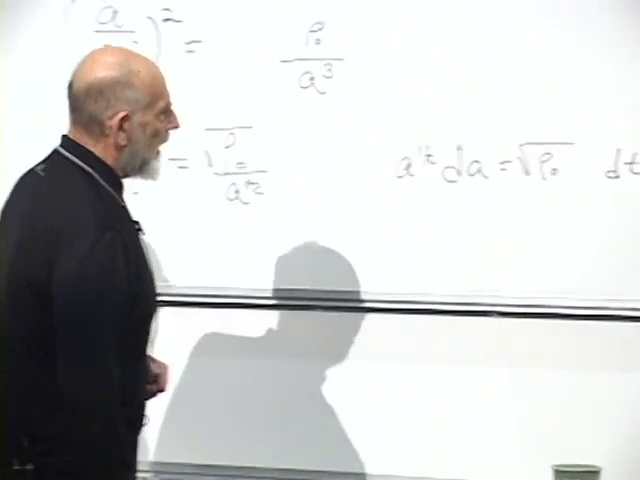
\includegraphics[width=0.86\textwidth]{lecture_08_figure_05.png}
\caption{物質密度の代入と変数分離により\(a^{1/2}da\propto dt\)が導かれる。}
\lectureframe{00:38:30.000}
\end{figure}

曲線\(t^{2/3}\)は直線よりもゆっくりと増加する。その傾きは減少するので、物質優勢宇宙は減速する。講義で用いられたニュートン的な言葉では、粒子は最初に離れ始め、それらの相互の重力引力が離れる割合を絶えず減少させる。

\begin{figure}[htbp]
\centering
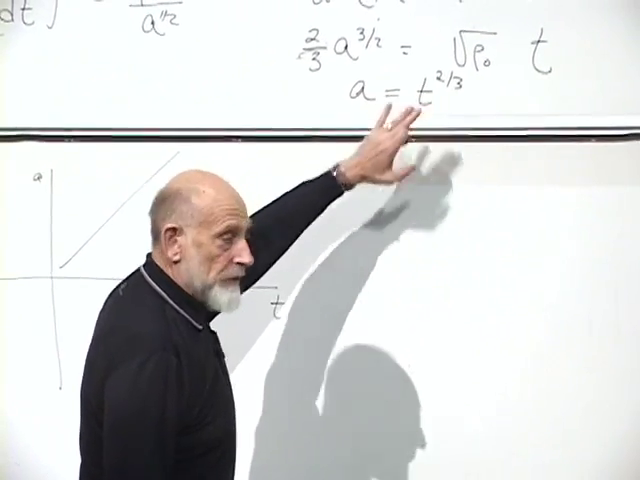
\includegraphics[width=0.86\textwidth]{lecture_08_figure_06.png}
\caption{線形膨張と下に凸な物質法則\(a(t)\propto t^{2/3}\)の黒板上での比較。}
\lectureframe{00:40:00.000}
\end{figure}

参考までに、放射浴は
\begin{equation}
\rho_r\propto a^{-4},
\end{equation}
であり、\(a^{-3}\)ではない。体積の希釈が三つの冪を寄与し、宇宙論的赤方偏移がもう一つ寄与する。対応するスケール因子も解くことができるが、講義ではその演習を意図的に脇に置いている。

\section{真空優勢膨張}

ここでフリードマン方程式の右辺に真空エネルギーのみを置く。\(\rho_{\rm vac}\)は定数であるから、
\begin{equation}
\left(\frac{\dot a}{a}\right)^2
=\frac{8\pi G_N}{3}\rho_{\rm vac}
\equiv H^2.
\label{eq:l08-de-sitter-friedmann}
\end{equation}
\(H\)の二つの用法を区別しておく必要がある。式~\eqref{eq:l08-hubble-definition}は時間に依存しうる量\(\dot a/a\)を定義する。式~\eqref{eq:l08-de-sitter-friedmann}は、純粋な真空エネルギー宇宙においてその値が定数
\begin{equation}
H=\sqrt{\frac{8\pi G_N\rho_{\rm vac}}{3}}.
\end{equation}
であることを述べている。膨張する枝を取ると
\begin{equation}
\dot a=Ha,
\end{equation}
となり、したがって
\begin{equation}
a(t)=C e^{Ht}.
\label{eq:l08-exponential-solution}
\end{equation}
となる。積分定数\(C\)は共動座標の任意の規格化を固定する。\(a\)の現在の値に比例する成長は指数関数的成長である。

\begin{figure}[htbp]
\centering
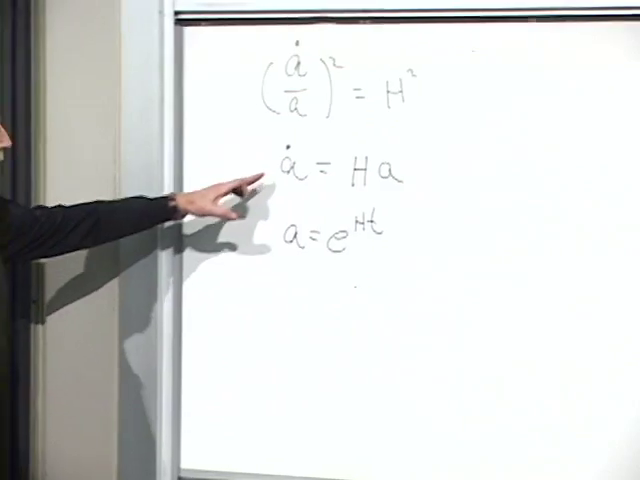
\includegraphics[width=0.88\textwidth]{lecture_08_figure_07.png}
\caption{真空優勢方程式\((\dot a/a)^2=H^2\)、その一階の形\(\dot a=Ha\)、および指数関数解。}
\lectureframe{00:47:45.000}
\end{figure}

共動物体に対するハッブル則は
\begin{equation}
v_{\rm rec}=HD.
\label{eq:l08-hubble-law}
\end{equation}
である。この純粋なド・ジッターの場合、後退速度が\(c\)に等しくなる固有距離は一定である。
\begin{equation}
D_H=\frac{c}{H},
\label{eq:l08-hubble-radius}
\end{equation}
または、黒板で用いられた\(c=1\)の単位では\(D_H=H^{-1}\)である。この固定されたスケールは、ド・ジッター事象の地平面半径として幾何学的に再び現れる。\editorialnote{ハッブル半径は、任意の時間依存宇宙論において自動的に事象の地平面となるわけではない。この同定がここで成り立つのは、厳密なド・ジッター空間において\(H\)が定数であるからである。}

この講義では、真空エネルギー検出器のための思考実験を提示する。他の源から遠く離れた、ごく軽い二つの試験体を、共動流に対して初め静止した状態に置き、それらの相互引力を無視できるようにする。それらの間隔は指数関数的膨張に従う。この効果は地上の装置にはあまりにも小さすぎるが、宇宙的距離と過去を見る時間によって、同じ物理が観測可能になる。

\section{物質支配から真空支配へ}

この講義で考察される実際の宇宙論的モデルには両方の項が含まれる：
\begin{equation}
H(t)^2
=\frac{8\pi G_N}{3}
\left(\frac{\rho_0}{a(t)^3}+\rho_{\rm vac}\right).
\label{eq:l08-mixed-friedmann}
\end{equation}
小さい\(a\)では、\(a^{-3}\)が大きいため物質項が支配し、解は\(t^{2/3}\)に似る。宇宙が成長するにつれて、物質は希薄化する一方で真空エネルギーは一定に留まる。やがて定数項が勝ち、スケール因子は\(e^{Ht}\)に向かって上向きに曲がる。

\begin{figure}[htbp]
\centering
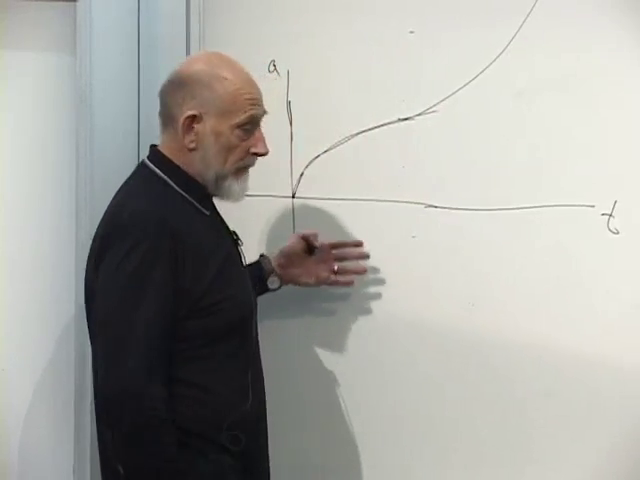
\includegraphics[width=0.87\textwidth]{lecture_08_figure_08.png}
\caption{この講義で描かれた定性的な転移：初期の物質支配による減速に続く、後期の真空支配による指数関数的成長。}
\lectureframe{00:53:30.000}
\end{figure}

\begin{classroomqa}
\audiencequestion{指数関数的解には積分定数が含まれる。それが極端に小さくないと、どうして分かるのか。\lecturetimestamp{00:52:41}}
\lecturerresponse{それを測定する。宇宙のより遠くを見ることは、より遠い過去を見ることを意味するので、異なる距離での観測は、膨張曲線の今日の値だけでなく、その初期部分を再構成する。}
\end{classroomqa}

この講義は、当時利用可能であった後期の観測が約5パーセントの水準で指数関数的な枝と整合していたと報告し、その証拠を説得力があると述べているが、電子の性質のような精密測定ほど厳密ではないとしている。これは現在の精密な主張としてではなく、講義当時の歴史的評価として読むべきである。

\begin{classroomqa}
\audiencequestion{上向きに曲がる膨張曲線は、最終的に我々が観測をビッグバンや宇宙マイクロ波背景放射まで遡ることを妨げるのか。\lecturetimestamp{00:55:05}}
\lecturerresponse{それはグラフの外挿に関する問題としては追及されない。関連する不変的な問題は事象の地平面の存在であり、それが今から扱う因果的な問題である。}
\end{classroomqa}

\section{束縛系と遠い未来}

指数関数的膨張が続くなら、希薄化するすべての成分は\(\rho_{\rm vac}\)に比べて無視できるようになる。これは、原子、太陽系、銀河それ自体が引き伸ばされるという意味ではない。束縛されたままでいるのに十分強く結びついた系はハッブル流に従わない。

\begin{classroomqa}
\audiencequestion{今日膨張していない銀河は、真空エネルギーが支配するようになると最終的に膨張するのか。\lecturetimestamp{00:57:44}}
\lecturerresponse{束縛系は束縛されたままである。天の川銀河とアンドロメダ銀河は、共に留まる近傍の構造に属するが、膨張とともにすでに運動している十分遠方の銀河は外へ進み続け、最終的に我々の地平面の向こうへと通過する。}
\end{classroomqa}

\emph{引き付けられている}ことと\emph{束縛されている}ことの区別は本質的である。脱出速度を超えて打ち上げられたロケットは地球の引力の下にあり続けるが、それでも戻ってこない。同様に、二つの銀河間の最大の局所的な力が通常の重力引力であっても、それらの相対軌道が束縛されているとは限らない。

\begin{classroomqa}
\audiencequestion{我々の銀河は重力によって集団と結びついている。加速膨張は最終的にその引力を打ち負かすのか。\lecturetimestamp{00:59:17}}
\lecturerresponse{局所構造の真に束縛された部分だけが共に留まる。銀河団という記述的なラベルだけでは十分ではない；束縛されているとは、相対運動が脱出以下にあることを意味する。より遠方の銀河は引き付けられていても、脱出速度を超えて後退することがある。}
\end{classroomqa}

直観のために、この講義は相対的な動径加速度を、引力の逆二乗項と間隔に線形な真空項の和として模式的に表す：
\begin{equation}
\ddot r\sim-\frac{G_NM}{r^2}+H^2r.
\label{eq:l08-newtonian-vacuum}
\end{equation}
理想化されたド・ジッター極限では係数は時間に依存しない。第二項が増大するのは\(r\)が増大するからだけであり、\(G_N\)が徐々に弱まることから生じるのではない。

\editorialnote{式~\eqref{eq:l08-newtonian-vacuum}はニュートン的な相対加速度のヒューリスティックであり、一般相対性理論に根本的な追加の力の法則ではない。厳密なド・ジッター空間では、隣接する自由落下世界線の相対加速度は\(H^2r\)に比例する。}

\begin{figure}[htbp]
\centering
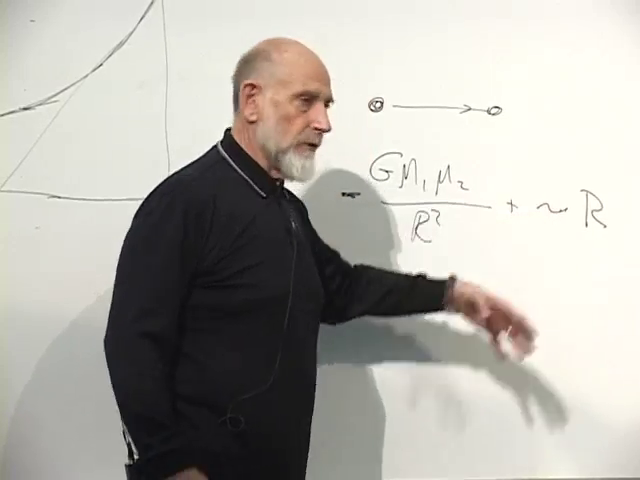
\includegraphics[width=0.88\textwidth]{lecture_08_figure_09.png}
\caption{逆二乗引力と、間隔に線形に増大する実効的な真空の斥力との黒板での比較。}
\lectureframe{01:04:10.000}
\end{figure}

\begin{classroomqa}
\audiencequestion{外向きの効果自体は時間とともに増大するのか。\lecturetimestamp{01:01:18}}
\lecturerresponse{固定した間隔では増大しない。その係数は一定である。自由に後退する物体は互いに遠ざかり、\(r\) に比例する項は、それらの距離が大きいために大きくなる。}
\end{classroomqa}

\begin{classroomqa}
\audiencequestion{正味の効果はニュートン定数の漸進的な減少として記述できるのか。\lecturetimestamp{01:02:30}}
\lecturerresponse{いいえ。\(G_N\) は一定のままである。指定された間隔では両方の係数は変わらず、\(1/r^2\) の引力と \(r\) に比例する項の相対的な重要性だけが距離とともに変化する。}
\end{classroomqa}

\begin{classroomqa}
\audiencequestion{真空エネルギーが重要になる前の初期宇宙において、同じ銀河は重力で束縛されていたのか。\lecturetimestamp{01:05:03}}
\lecturerresponse{通常の引力が支配的であること自体は、束縛を意味しない。多くの銀河はすでに脱出速度程度かそれ以上で互いに離れつつあった。真空エネルギーは後に、大規模な膨張が再収縮に向かって減速するか、それとも加速して遠ざかるかを決めるが、最大の力と束縛軌道は別の主張である。}
\end{classroomqa}

したがって、遠い未来の観測者は、合体した局所構造の中に住む一方で、束縛されていないすべての銀河は観測不可能になっているかもしれない。歴史的記録がなければ、その観測者はほとんど空の宇宙を推論しても妥当であろう。この因果的な孤独こそが、局所的な物体の破壊ではなく、地平線への物理的な導入である。

\section{事象の地平線が意味するもの}

休憩の後、
\begin{equation}
a(t)=e^{Ht}
\end{equation}
と置き、計量を
\begin{equation}
ds^2=-dt^2+e^{2Ht}d\mathbf{x}^2.
\label{eq:l08-de-sitter-metric}
\end{equation}
と書く。

\begin{classroomqa}
\audiencequestion{この計量が記述する時空の名前は何か。\lecturetimestamp{01:08:13}}
\lecturerresponse{それはド・ジッター時空であり、通常はド・ジッター空間と略される。その地平線が重要であるのは、真空が支配的な宇宙が後期にこの幾何学に近づくからである。}
\end{classroomqa}

その因果構造を描く前に、ペンローズ図の役割を思い出そう。無限の区間は、ヌル光線が \(45^\circ\) にとどまるまま、有限の図に圧縮される。平坦な時空では、質量をもつ物体は未来の時間的無限遠で終わり、ヌル光線はヌル無限遠で終わり、任意に長く待つことを許された慣性観測者には、時空の永続的な領域を排除する事象の地平線は存在しない。

\begin{figure}[htbp]
\centering
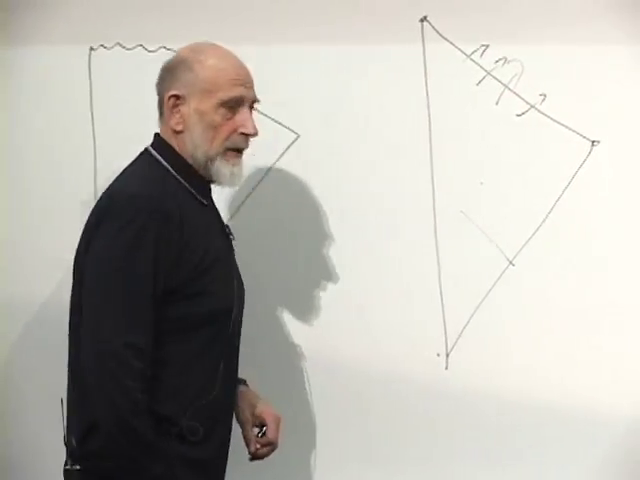
\includegraphics[width=0.80\textwidth]{lecture_08_figure_10.png}
\caption{地平線を導入する前に、時間的およびヌルの行き先を区別するために用いられる平坦時空のペンローズ図。}
\lectureframe{01:10:35.000}
\end{figure}

ブラックホールの図は対照を与える。外部の観測者は、観測者の未来の世界線の因果的過去にある事象からのみ信号を受け取ることができる。観測時間が無限大に近づいても、内部領域は排除されたままである。その観測者と通信できる事象と決してできない事象との境界が事象の地平線である。

\begin{definition}
観測者の未来の事象の地平線とは、未来向きの因果的信号がその観測者の世界線にいつか到達しうる事象の集合の境界である。
\label{def:l08-event-horizon}
\end{definition}

\begin{figure}[htbp]
\centering
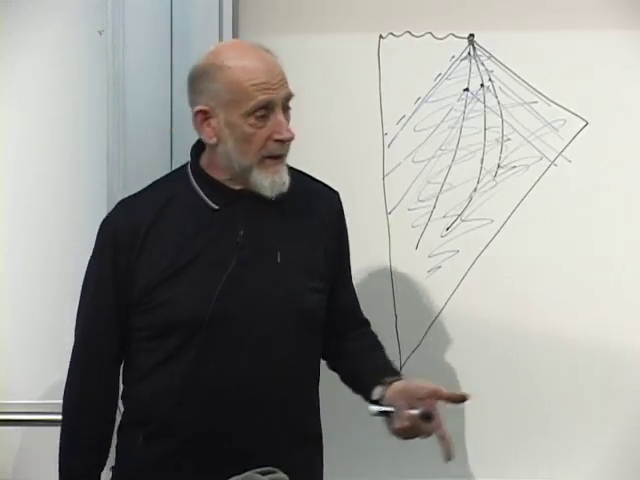
\includegraphics[width=0.80\textwidth]{lecture_08_figure_11.png}
\caption{ブラックホールとの比較：任意に遅い外部観測からの過去光円錐は、事象の地平線の向こう側の領域を決して含まない。}
\lectureframe{01:13:50.000}
\end{figure}

したがって事象の地平線は大域的な因果的境界であり、単に物体が今日たまたま暗く見える距離ではない。それを特定するには、任意に長く待った後でもどの信号が到達しうるかを知らなければならない。

\section{無限の未来を圧縮する}

式~\eqref{eq:l08-de-sitter-metric} の空間座標はすでに無限の平坦なスライスにわたっている。それらはそのままにし、時間だけを圧縮する。共形時間 \(T\) を
\begin{equation}
dt^2=e^{2Ht}dT^2.
\label{eq:l08-conformal-definition}
\end{equation}
を要求することによって導入する。未来向きの平方根をとり、整理すると
\begin{equation}
dT=e^{-Ht}dt.
\end{equation}
が得られる。

\begin{classroomqa}
\audiencequestion{符号を含め、その積分は何か。\lecturetimestamp{01:17:25}}
\lecturerresponse{それは \(-H^{-1}e^{-Ht}\) である。付加定数は \(T\) の原点をずらすだけなので、無限の未来を \(T=0\) に置くように選ぶ。}
\end{classroomqa}

したがって
\begin{equation}
T=-\frac{1}{H}e^{-Ht},
\qquad -\infty<T<0.
\label{eq:l08-conformal-time}
\end{equation}
\(t\to-\infty\) のとき、\(T\to-\infty\)。固有時間 \(t\to+\infty\) のとき、\(T\to0^{-}\)。無限の未来は有限の水平線 \(T=0\) 上に置かれた。どの観測者も有限の固有時間ではそこに到達しない。

\begin{figure}[htbp]
\centering
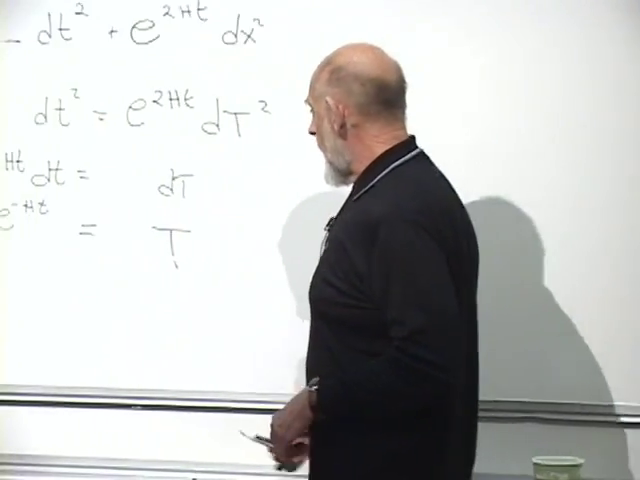
\includegraphics[width=0.86\textwidth]{lecture_08_figure_12.png}
\caption{共形時間の積分と、無限の未来 \(t\to+\infty\) の \(T=0^{-}\) への写像。}
\lectureframe{01:19:10.000}
\end{figure}

式~\eqref{eq:l08-conformal-time} から、
\begin{equation}
HT=-e^{-Ht},
\qquad
e^{2Ht}=\frac{1}{H^2T^2}.
\label{eq:l08-conformal-factor}
\end{equation}
式~\eqref{eq:l08-de-sitter-metric} で \(dt=e^{Ht}dT\) を用いると、
\begin{equation}
ds^2=\frac{1}{H^2T^2}
\left(-dT^2+d\mathbf{x}^2\right).
\label{eq:l08-conformal-metric}
\end{equation}
が得られる。括弧内の表式はミンコフスキー計量である。ド・ジッター幾何学はすべて、\(T\to0^{-}\) のとき発散する共通の共形因子の中に入っている。

\begin{figure}[htbp]
\centering
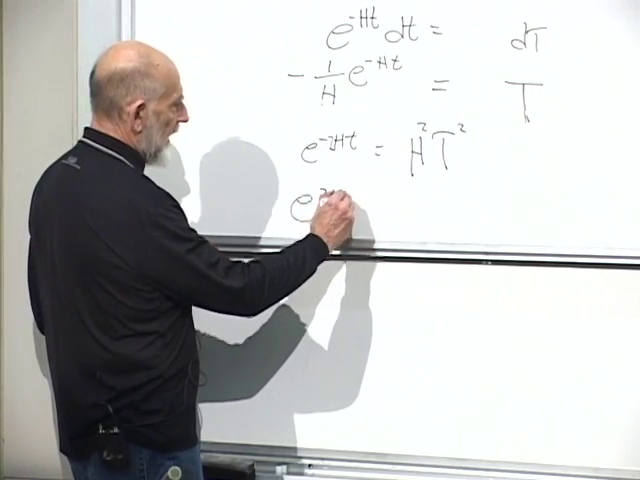
\includegraphics[width=0.87\textwidth]{lecture_08_figure_13.png}
\caption{\(e^{2Ht}\) を \(1/(H^2T^2)\) に関係づけ、計量の共形形を準備する代数。}
\lectureframe{01:22:50.000}
\end{figure}

\begin{classroomqa}
\audiencequestion{この計量において、光線の経路はどのような条件で決まるのですか。\lecturetimestamp{01:23:49}}
\lecturerresponse{光線はヌル経路 \(ds^2=0\) に従う。したがって共通の共形因子は相殺され、選んだ空間方向に沿って \(dT=\pm dx\) が残る。}
\end{classroomqa}

光線は \((T,x)\) 図において \(45^\circ\) の直線である：
\begin{equation}
\frac{dx}{dT}=\pm1.
\label{eq:l08-null-lines}
\end{equation}
座標による描像は \(T=0\) の近くでひどく圧縮されているが、必要なこと、すなわちどの事象が通信できるかを正確に保っている。

\begin{figure}[htbp]
\centering
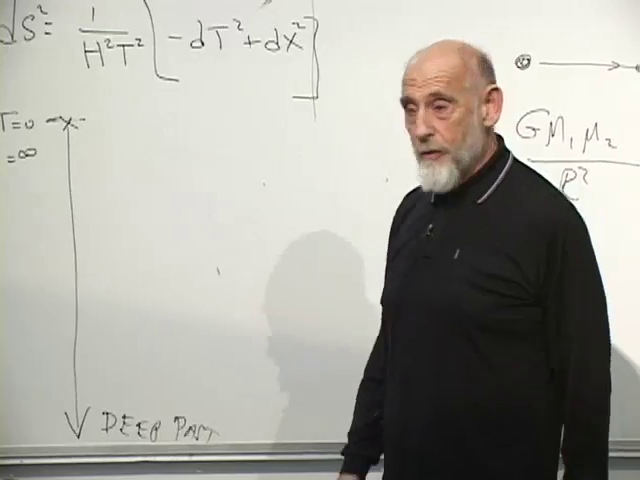
\includegraphics[width=0.86\textwidth]{lecture_08_figure_14.png}
\caption{ヌル条件 \(ds^2=0\) を用いて \(45^\circ\) の光線を回復する時点での共形計量。}
\lectureframe{01:24:05.000}
\end{figure}

\section{ド・ジッター空間におけるアリスとボブ}

アリスを固定された共動位置 \(x=0\) に置く。彼女の世界線は垂直に上昇し、図の上では \(T=0\) で終わるが、彼女の腕時計がそこに到達するには無限の固有時間を要する。その端点から過去向きのヌル光線を引く。それらはアリスが信号を受け取ることのできる最大の領域を境界づける。その外側の事象は永遠に到達不能のままである。

\begin{figure}[htbp]
\centering
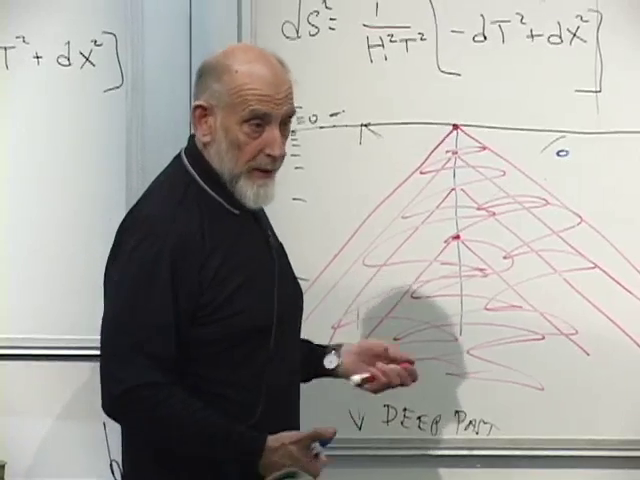
\includegraphics[width=0.88\textwidth]{lecture_08_figure_15.png}
\caption{アリスの限界的な過去光円錐。そのヌル境界が、観測者に依存する彼女のド・ジッター事象の地平面である。}
\lectureframe{01:28:50.000}
\end{figure}

この地平面は私的なものである。異なる観測者は異なる未来の端点を持ち、したがって異なる限界的な過去光円錐を持つ。かつてボブがアリスの因果的領域内にあり、二人がメッセージを交換したとしよう。その後ボブがハッブル流に従ってアリスの地平面を越えると、その越境後に発せられた信号は、アリスがどれほど待っても彼女に届かない。ボブは自分自身の地平面を持ち、やがてアリスからの遅い信号を受け取るという対応する能力を失う。

\begin{figure}[htbp]
\centering
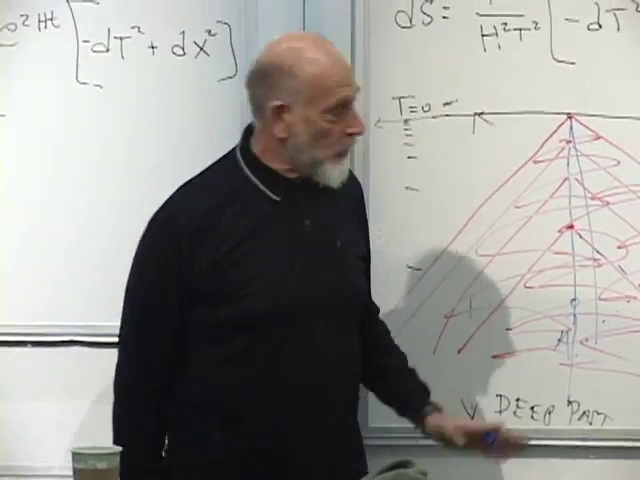
\includegraphics[width=0.88\textwidth]{lecture_08_figure_16.png}
\caption{アリスとボブ、それぞれ異なる因果的境界を持つ。共動するボブは、以前に信号を交換していたとしても、アリスの因果的過去から離れることができる。}
\lectureframe{01:30:20.000}
\end{figure}

アリスとボブが手をつなぐ、あるいはより現実的には固定された固有間隔で束縛され続けるなら、彼らの共動座標の間隔は \(a^{-1}\) として縮む。彼らの曲線は共形図において互いに近づくが、これは彼らの固有距離が消えることを意味しない。増大する共形因子が縮む座標の隔たりを補償し、通信はいつまでも可能なままである。

\begin{classroomqa}
\audiencequestion{地平面が二人を隔てた後、ボブはアリスを同時に見ることができますか。\lecturetimestamp{01:31:43}}
\lecturerresponse{いかなる観測者も、その文字通りの意味で遠方の事象を同時に見ることはない。観測とは常に過去光円錐内の事象についてのものである。より鋭い言明は、地平面の越境後には、もう一方の世界線から新たに発せられた信号は到着し得ないということである。}
\end{classroomqa}

遠い未来の宇宙論的応用では、アリスは我々の束縛された局所的な残存物を表し、ボブはそれぞれの束縛されていない遠方の銀河を表す。銀河はアリスの時計上の有限の瞬間に突然消えるのではない。それらの後の信号はより長い間隔に引き伸ばされ、より長い波長へとずれ、ついには物理的に検出不能になる。

\begin{classroomqa}
\audiencequestion{理論は本当に、遠い未来にはもはや可視の遠方銀河は残らないと言うのですか。\lecturetimestamp{01:33:38}}
\lecturerresponse{束縛されていない銀河は局所観測者の事象の地平面の向こうへと過ぎ去る。それらの最後の可視信号はますます遅延し赤方偏移し、実用上は束縛された局所構造のみが観測可能なまま残る。}
\end{classroomqa}

\section{地平面における赤方偏移}

ボブからの古い光信号が非常に遅い共形時間にアリスに到達する様子を描くことは依然としてでき、それによって彼女が彼を見続けているように見せかけることができる。物理的内容はそれらの信号の間隔とエネルギーにある。ボブの時計の等しい間隔は、アリスの固有時間のますます大きな間隔を隔てて到着する。振動数と光子エネルギーは低下する：
\begin{equation}
\nu_{\rm received}\longrightarrow0,
\qquad
E_{\rm received}=h\nu_{\rm received}\longrightarrow0.
\end{equation}
ボブの像は遅くなり、赤くなり、薄れる。極限の信号は消えゆく有用な情報しか運ばない。

\begin{figure}[htbp]
\centering
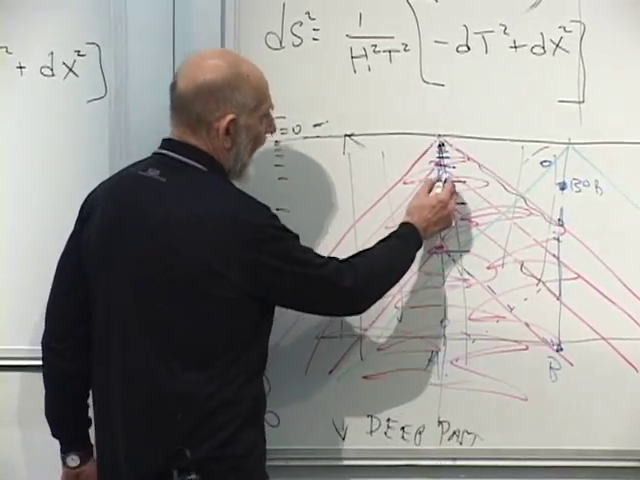
\includegraphics[width=0.89\textwidth]{lecture_08_figure_17.png}
\caption{ド・ジッター地平面の赤方偏移と、ブラックホール地平面のよく知られた外部からの見え方を比較した、後半の板書状態。}
\lectureframe{01:36:20.000}
\end{figure}

\begin{classroomqa}
\audiencequestion{これはブラックホールの場合、すなわち外部の観測者が落下する物体が地平面を越えるのを決して見ないのと同じですか。\lecturetimestamp{01:36:09}}
\lecturerresponse{はい。どちらの場合も、観測者はますます赤方偏移した信号を受け取り、越境が完了するのを直接見ることは決してない。因果図はどの後の放出が決して到着し得ないかを語り、赤方偏移は最後の観測可能な情報がどのように薄れるかを説明する。}
\end{classroomqa}

この類推は温度についての問いを促す。

\begin{classroomqa}
\audiencequestion{アリスはどうやって地平面のすぐ上の温度を測定できるのだろうか。\lecturetimestamp{01:39:34}}
\lecturerresponse{操作上は、ケーブルで温度計を降ろし、地平面を越えないように保ち、そして引き戻せばよい。ド・ジッター観測者は宇宙論的地平面の近くで同様の実験を想像できる。量子論では地平面は熱いが、本講義は古典幾何学で止まり、その計算は先送りにする。}
\end{classroomqa}

ここではド・ジッター温度の公式は導出されない。ホーキング放射は、この古典的描像に対する量子補正の予告としてのみ登場する。

\section{固定された地平面半径}

共形図は元の時間座標に翻訳し直すことができる。固定された座標間隔にある2つの共動点は
\begin{equation}
D(t)=e^{Ht}\lvert\Delta x\rvert,
\end{equation}
を満たすので、それらの固有距離は指数的に増大する。

\begin{classroomqa}
\audiencequestion{同じ運動は、変換前の元の時間座標ではどのように見えるだろうか。\lecturetimestamp{01:41:14}}
\lecturerresponse{固定された共動座標に対して、空間計量全体が\(e^{2Ht}\)とともに増大する。したがって固有間隔は\(e^{Ht}\)のように増大する。座標変換を元に戻すと、その膨張が明示的になる。}
\end{classroomqa}

地平面は異なる振る舞いをする。なぜなら、アリスからの共動座標距離は固定されていないからである。\(T=0\)で終わる\(45^\circ\)のヌル線から、一定の\(T<0\)のスライス上での地平面距離は
\begin{equation}
\Delta x_H=-T=\frac{1}{H}e^{-Ht}.
\label{eq:l08-coordinate-horizon}
\end{equation}
であり、スケール因子を掛けると
\begin{equation}
D_H(t)=a(t)\Delta x_H
=e^{Ht}\frac{e^{-Ht}}{H}
=\frac{1}{H}.
\label{eq:l08-fixed-horizon}
\end{equation}
となる。単位を戻すと、\(D_H=c/H\)である。座標間隔は縮み、計量スケールは成長し、それらの積は一定に保たれる。

\begin{classroomqa}
\audiencequestion{時間が経つにつれて、アリスから地平面までの距離は増大するだろうか、縮小するだろうか、それとも同じままであるだろうか。\lecturetimestamp{01:42:42}}
\lecturerresponse{同じままである。その座標距離は縮む一方で共形因子が成長し、\(c=1\)とする単位で固有地平面半径は\(H^{-1}\)に固定されたままである。}
\end{classroomqa}

\begin{figure}[H]
\centering
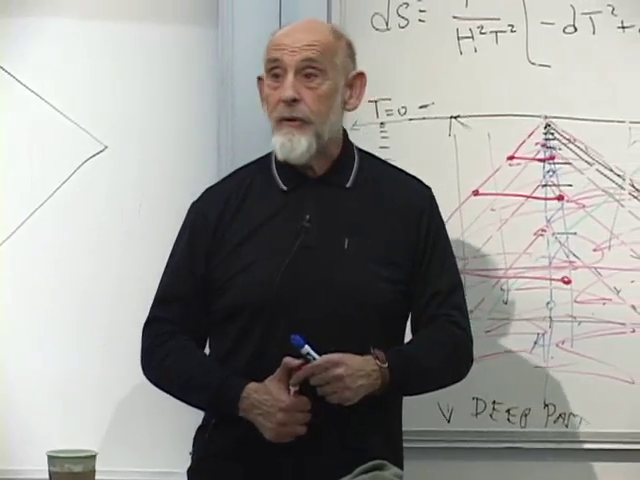
\includegraphics[width=0.90\textwidth]{lecture_08_figure_18.png}
\caption{最終的な板書の状態：連続する水平スライスでは、地平面までの座標距離は縮小するが、固有距離は同じである。}
\lectureframe{01:43:20.000}
\end{figure}

\begin{classroomqa}
\audiencequestion{古い像が決して完全には消えないために、アリスは過去が地平面に投影されたものを見続けるのだろうか。\lecturetimestamp{01:43:45}}
\lecturerresponse{古典的には、それらの像は、無限に続く赤方偏移によってますます検出しにくくなるという極限的な意味でのみ持続する。この記述は、地平面に付随するホーキング放射を省いており、それが量子論的記述を変更するだろう。}
\end{classroomqa}

したがって講義は、正確な境界で終わる。真空エネルギーが指数的膨張を生み、指数的膨張が固定された観測者依存の事象の地平面を生み、そしてその地平面の近くの信号は振動数がゼロになるまで追いやられた。地平面の温度とホーキング放射は次に来るものに属する。ススキンドが言うように、我々が互いの地平面を横切らないと仮定すれば、次の講義でまた会おう。
